\documentclass[11pt,reqno,final]{amsart}

\pdfcompresslevel=0
\pdfobjcompresslevel=0

\usepackage[dvipsnames]{xcolor}% adds colors
\usepackage{amsmath, amsthm}% {amsfonts, amssymb}

% New Characters
\usepackage[latin1]{inputenc}%
\usepackage[T1]{fontenc}

\usepackage{MnSymbol}
\usepackage[normalem]{ulem}% underlining

\usepackage[theoremfont, largesc]{newpxtext} % different text,math font
\usepackage{newpxmath}

\makeatletter
\DeclareMathRadical{\sqrtsign}{symbols}{112}{largesymbols}{112}
\let\sqrt=\undefined
\DeclareRobustCommand\sqrt{\@ifnextchar[\@sqrt{\mathpalette\@x@sqrt}]}
\def\@x@sqrt#1#2{%
 \setbox\z@\hbox{$\m@th#1\sqrtsign{\mkern1mu #2}$}
 \mkern3mu\box\z@}
\makeatother




% Page Typesetting
\usepackage[final]{microtype}
\usepackage{relsize}
\usepackage[margin=1in]{geometry}
\usepackage{framed}
\usepackage{tikz}
\usepackage{setspace}

\usepackage{hyperref}
\hypersetup{
  final,
  pdftitle={Math 135 - Limits},
  pdfauthor={Bonventre}, 
  linktoc=page,
  pagebackref,
  colorlinks=true,
  citecolor=PineGreen,
  linkcolor=PineGreen,
  linkbordercolor=PineGreen,
}


% Internal References

\usepackage[inline,shortlabels]{enumitem}

\numberwithin{equation}{section} 
\numberwithin{figure}{section}

\usepackage[nameinlink,capitalise,noabbrev]{cleveref}

\crefname{equation}{}{} % get \cref to behave as \eqref

% \theoremstyle{plain} % bold name, italic text
\newtheorem{theorem}[equation]{Theorem}%
\newtheorem*{theorem*}{Theorem}%
\newtheorem{lemma}[equation]{Lemma}%
\newtheorem{proposition}[equation]{Proposition}%
\newtheorem{corollary}[equation]{Corollary}%
\newtheorem{conjecture}[equation]{Conjecture}%
\newtheorem*{conjecture*}{Conjecture}%
\newtheorem{claim}[equation]{Claim}%
\newtheorem{question}{Question}

\theoremstyle{definition} % bold name, plain text
\newtheorem{definition}[equation]{Definition}%
\newtheorem*{definition*}{Definition}%
\newtheorem{example}[equation]{Example}%
\newtheorem*{example*}{Example}%
\newtheorem{remark}[equation]{Remark}%
\newtheorem{notation}[equation]{Notation}%
\newtheorem{convention}[equation]{Convention}%
\newtheorem{assumption}[equation]{Assumption}%
\newtheorem{exercise}[question]{Exercise}

% ---------- macros
\newcommand{\set}[1]{\left\{#1\right\}}%
\newcommand{\sets}[2]{\left\{ #1 \;|\; #2\right\}}%
\newcommand{\longto}{\longrightarrow}%
\newcommand{\into}{\hookrightarrow}%
\newcommand{\onto}{\twoheadrightarrow}%

\usepackage{harpoon}
\newcommand{\vect}[1]{\text{\overrightharp{\ensuremath{#1}}}}

\newcommand{\del}{\partial}%

\newcommand{\ki}{\chi}
\newcommand{\ksi}{\xi}
\newcommand{\Ksi}{\Xi}

% %%%%%%%%%%%%%%%%%%%%%%%%%%%%%%%%%%%%%%%%%%%%%%%%%%%%%%%%%%%%%%%%%%%%%%%%%%%%%%%%%%%%%%%%%%%%%%%%%%%%

\begin{document}
\onehalfspacing

\begin{center}
        \textbf{\Large Math 135, Calculus 1, Fall 2020}\\[10pt]
        {\large 09-16: Limits, Velocity, and Tangent Lines}
\end{center}

\thispagestyle{empty}

\renewcommand{\thesection}{\Alph{section}}

\section{Limits}

\begin{definition*}
        Given a function $f(x)$, we say that \textit{the limit of $f(x)$ as $x$ approaches $c$ is equal to the number $L$} if
        $|f(x)-L|$ can be made arbitrarily small by taking $x$ sufficiently close (but not equal) tto $c$.

        In this case, we write
        \[
                \lim_{x \to c}f(x) = L
        \]
        and say ``$f(x)$ approaches $L$ as $x$ goes to $c$''.
        \begin{center}
                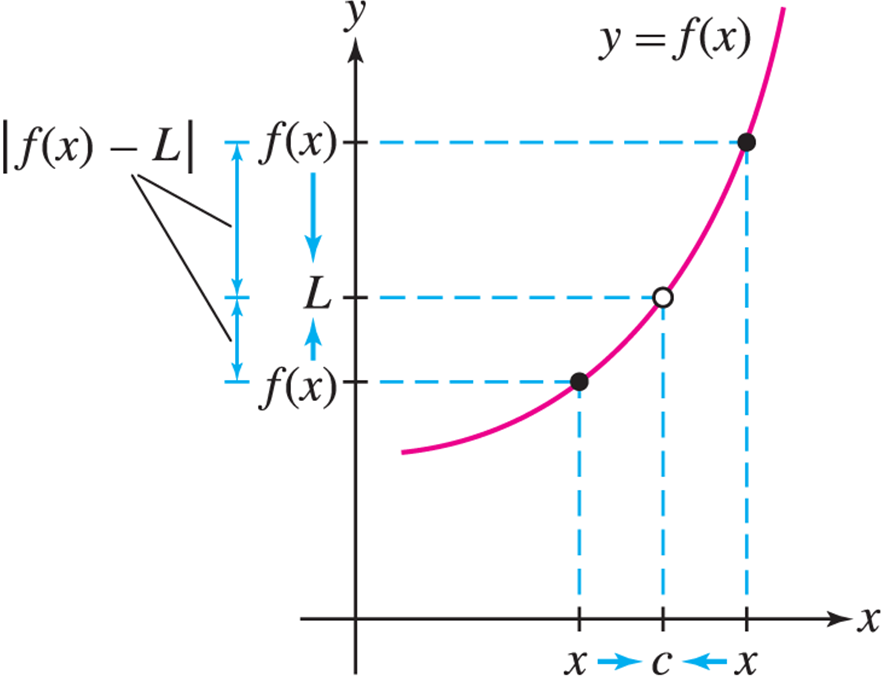
\includegraphics[width=2.5in]{09-16P-lim.png}
        \end{center}
\end{definition*}

\begin{example*}
        On Wednesday, in Exercise 2, we numerically computed/estimated that
        \[
                \lim_{t \to 1}\dfrac{t^2+4t-5}{t-1} = 6.
        \]
        Note that, even though $\frac{t^2+4t-5}{t-1}$ is \textbf{not defined} at $t = 1$ (can't divide by 0), \textit{the limit still exists}.
        We only care about the value that the function \textbf{approaches} as we get close to the point in question.
        The actual value of the function (or lack thereof) at the destination point is irrelevant.
\end{example*}

\begin{exercise}
        Using the graph of $f(x)$ below, compute $\displaystyle\lim_{x \to 1} f(x)$ and $\displaystyle\lim_{x \to 4}f(x)$.

        $ $\\
        
        \begin{minipage}{.5\textwidth}
                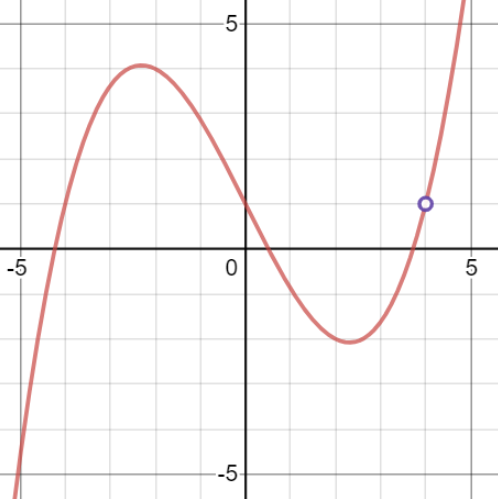
\includegraphics[width=2.5in]{09-18P_hole.png}
        \end{minipage}
        \begin{minipage}{.5\textwidth}
                $ $
        \end{minipage}
\end{exercise}

\newpage

\subsection{One-sided limits}

Consider the function below. As $x$ gets closer to 4, the function values approach two \textit{different} quantities, depending on which direction $x$ approaches 4 from:
\begin{itemize}
\item the \textbf{left-hand limit} at $x = 4$ (approaching from the left, $x<4$) is $3$
\item the \textbf{right-hand limit} at $x = 4$ (appraoching from the right, $x>4$) is $1$.
\end{itemize}
\begin{minipage}{.5\textwidth}
        $ $\\
        \begin{center}
                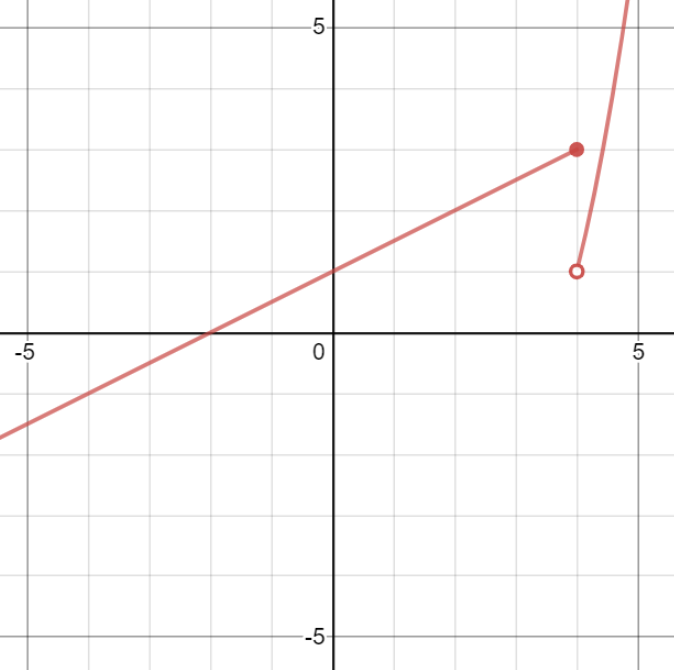
\includegraphics[width=2.5in]{09-18P_jump.png}
        \end{center}        
\end{minipage}
\begin{minipage}{.5\textwidth}
        We write\\
        
        \textbf{Left-hand limit:}\quad $\displaystyle\lim_{x \to 4^-}f(x) = 3$\\[10pt]
        
        \textbf{Right-hand limit:}\quad $\displaystyle\lim_{x \to 4^+}f(x) = 1$
\end{minipage}

In this case, the limit $\displaystyle\lim_{x \to 4}f(x)$ \textbf{does not exist}, since the left- and right-hand limits do not agree.

\begin{framed}
        \[
                \displaystyle\lim_{x \to a}f(x) = L \mbox{ if and only if } \displaystyle\lim_{x \to a^-} f(x) = L \mbox{ and } \lim_{x \to a^+}f(x) = L.
        \]
\end{framed}

\begin{exercise}
        Evaluate each of the following using the graph of $g(x)$ shown below.\\

        \begin{minipage}{.5\textwidth}
                \begin{enumerate}[(a)]\itemsep+7pt
                \item $\displaystyle\lim_{x \to -1^-} g(x)$\\
                \item $\displaystyle\lim_{x \to -1^+} g(x)$\\
                \item $\displaystyle\lim_{x \to -1} g(x)$\\
                \item $g(-1)$\\
                \item $\displaystyle\lim_{x \to 1^-} g(x)$\\
                \item $\displaystyle\lim_{x \to 1^+} g(x)$\\
                \item $\displaystyle\lim_{x \to 1} g(x)$\\
                \item $g(1)$
                \end{enumerate}
        \end{minipage}
        \begin{minipage}{.5\textwidth}
                $ $\\

                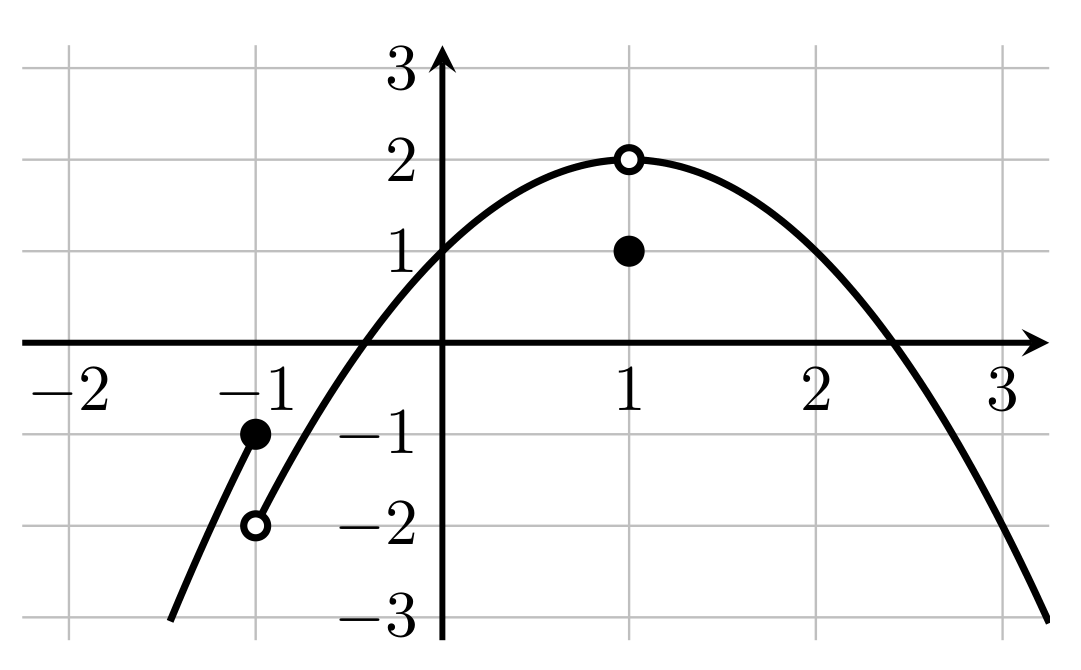
\includegraphics[width=3in]{09-18P_ex.png}
        \end{minipage}
\end{exercise}

\newpage

\subsection{Infinite Limits}

It may happen that as $x$ approaches the value $a$, the function value increases (or decreases) without bound.
In these cases, we say that the limit is $\infty$ (or $-\infty$).

(\textbf{Warning:} These limits still \textbf{do not exist}. However, we can be precise about how they don't exist.)

\begin{exercise}
        Compute each of the following limits. It may help to think qualitatively, e.g. ``What happens as $x$ is very close, but slightly smaller, than $3$?''\\
        \begin{enumerate}[(a)]\itemsep+35pt
        \item $\displaystyle\lim_{x \to 3^-} \dfrac{1}{x-3}$
        \item $\displaystyle\lim_{x \to 3^+} \dfrac{1}{x-3}$
        \item $\displaystyle\lim_{x \to 3} \dfrac{1}{x-3}$
        \item $\displaystyle\lim_{x \to 0^-} \ln x$
        \end{enumerate}

       
\end{exercise}
\end{document}
